\section{12 Oct 23 - Activity: Method of
Relaxation}\label{oct-23---activity-method-of-relaxation}

As we discussed, we can use the relaxation approach to solve Laplace's
equation. As a reminder the process for doing this is as follows:

\begin{enumerate}
\def\labelenumi{\arabic{enumi}.}
\tightlist
\item
  Divide the region into a grid
\item
  Set the boundary conditions on the edges of the grid
\item
  Guess the starting values for the potential in the interior of the
  grid (not on the edges)
\item
  Calculate the potential at each point in the grid using the average of
  the neighboring points (replacing the value as you go)
\item
  Repeat step 4 until the values in the grid stops changing
\end{enumerate}

Below, we have written up a 1D code that performs each of these steps.
Your task is to modify this code to work in 2D. You will need to write
the functions that compute the potential at each point in the 2D grid as
well as the function that sets the boundary conditions.

\begin{Shaded}
\begin{Highlighting}[]
\ImportTok{import}\NormalTok{ numpy }\ImportTok{as}\NormalTok{ np}
\ImportTok{import}\NormalTok{ matplotlib.pyplot }\ImportTok{as}\NormalTok{ plt}
\end{Highlighting}
\end{Shaded}

\subsection{1 Dimensional Relaxation}\label{dimensional-relaxation}

The 1D problem is rather simple in that it produces a linear function --
always. This is because the only solution to the 1D Laplace's equation
is a linear function.

\[\frac{d^2V}{dx^2} = 0\]

The solution to this equation is \(V(x) = ax + b\). We can use this to
test our relaxation code and make sure that it is accurate. In general,
you cannot do this and instead need to have some other mechanism for
checking the accuracy of your code (like
\href{https://en.wikipedia.org/wiki/Rate_of_convergence}{convergence}).

Below, we have written the 1D code as a set of functions.

\subsubsection{Initialize the Grid and set the Boundary
Conditions}\label{initialize-the-grid-and-set-the-boundary-conditions}

We wrote two functions \texttt{initialize\_grid} and
\texttt{set\_boundary\_conditions} that initialize a linear grid and
also set the boundary conditions. The \texttt{initialize\_grid} function
simply sets all values to zero and then
\texttt{set\_boundary\_conditions} sets the values at the edges to the
correct values.

\begin{Shaded}
\begin{Highlighting}[]
\KeywordTok{def}\NormalTok{ initialize\_grid(size):}
    \CommentTok{\#\# Set the initial values of the grid}
    
    \ControlFlowTok{return}\NormalTok{ np.zeros(size)}

\KeywordTok{def}\NormalTok{ set\_boundary\_conditions(grid, left\_val, right\_val):}
    \CommentTok{\#\# Set the boundary conditions}
\NormalTok{    grid[}\DecValTok{0}\NormalTok{] }\OperatorTok{=}\NormalTok{ left\_val}
\NormalTok{    grid[}\OperatorTok{{-}}\DecValTok{1}\NormalTok{] }\OperatorTok{=}\NormalTok{ right\_val}
    
    \ControlFlowTok{return}\NormalTok{ grid}
\end{Highlighting}
\end{Shaded}

\subsubsection{Relaxation}\label{relaxation}

The core relaxation function is \texttt{run\_relaxation}. Notice that it
takes in the number of iterations (\texttt{num\_iterations}); that is,
the number of times you want the relaxation algorithm to run. That is,
it will calculate the average of the neighboring points fully, and
repeat it a limited number of times.

\textbf{This is not how the typical relaxation approach works.}

Normally, you would run the algorithm until the changes between each
iteration are below some error tolerance you've chosen. This can lead to
(near)infinite loops if your approach: (1) doesn't converge or (2)
converges very slowly. So it is important to have a maximum number of
iterations to run. \textbf{You will modify the 1D code to do this.}

Notice that our relaxation function stores the values of the potential
at set iterations (\texttt{store\_freq}). This is to allow us to plot
the potential at different points in the relaxation process. But we
don't want to keep them all as that can become memory intensive.

\begin{Shaded}
\begin{Highlighting}[]

\KeywordTok{def}\NormalTok{ run\_relaxation(grid, num\_iterations, store\_freq}\OperatorTok{=}\DecValTok{500}\NormalTok{):}
    \CommentTok{\#\# Run the relaxation algorithm}
    \CommentTok{\#\# Store the grid at regular intervals}
\NormalTok{    stored\_iterations }\OperatorTok{=}\NormalTok{ []}
    
    \CommentTok{\#\# Run the relaxation}
    \ControlFlowTok{for}\NormalTok{ i }\KeywordTok{in} \BuiltInTok{range}\NormalTok{(num\_iterations):}
        \ControlFlowTok{for}\NormalTok{ j }\KeywordTok{in} \BuiltInTok{range}\NormalTok{(}\DecValTok{1}\NormalTok{, }\BuiltInTok{len}\NormalTok{(grid)}\OperatorTok{{-}}\DecValTok{1}\NormalTok{):}
            \CommentTok{\#\# Update the grid point with the average of the neighboring points}
\NormalTok{            grid[j] }\OperatorTok{=} \FloatTok{0.5} \OperatorTok{*}\NormalTok{ (grid[j}\OperatorTok{{-}}\DecValTok{1}\NormalTok{] }\OperatorTok{+}\NormalTok{ grid[j}\OperatorTok{+}\DecValTok{1}\NormalTok{])}
        
        \CommentTok{\#\# Store the grid every store\_freq iterations}
        \ControlFlowTok{if}\NormalTok{ i }\OperatorTok{\%}\NormalTok{ store\_freq }\OperatorTok{==} \DecValTok{0}\NormalTok{:}
\NormalTok{            stored\_iterations.append(np.copy(grid))}
    
    \ControlFlowTok{return}\NormalTok{ stored\_iterations}
\end{Highlighting}
\end{Shaded}

\subsubsection{Plotting}\label{plotting}

Our relaxtion algorithm stores a list of grids at different points in
the relaxation process. We can use this to plot the potential at
different points. Below, we have a function that does just that.

\begin{Shaded}
\begin{Highlighting}[]

\KeywordTok{def}\NormalTok{ plot\_results(stored\_iterations):}
    \CommentTok{\#\# Plot the results (including all stored iterations)}
    \ControlFlowTok{for}\NormalTok{ i, grid }\KeywordTok{in} \BuiltInTok{enumerate}\NormalTok{(stored\_iterations):}
\NormalTok{        plt.plot(grid, label}\OperatorTok{=}\SpecialStringTok{f"Iteration }\SpecialCharTok{\{}\NormalTok{i}\OperatorTok{*}\NormalTok{store\_freq}\SpecialCharTok{\}}\SpecialStringTok{"}\NormalTok{)}
\NormalTok{    plt.legend()}
\NormalTok{    plt.xlabel(}\StringTok{\textquotesingle{}Grid Index\textquotesingle{}}\NormalTok{)}
\NormalTok{    plt.ylabel(}\StringTok{\textquotesingle{}Potential\textquotesingle{}}\NormalTok{)}
\NormalTok{    plt.title(}\StringTok{\textquotesingle{}1D Relaxation\textquotesingle{}}\NormalTok{)}
\NormalTok{    plt.show()}
\end{Highlighting}
\end{Shaded}

\subsubsection{Let's run it}\label{lets-run-it}

We run the code below for linear grid of 100 points. The left boundary
condition (\(x=0\)) is set to zero and the right one (\(x=a\)) is set to
10. Notice that there is an exact solution:

\[V(x) = 10\frac{x}{a}\]

We can compare to that exact solution to see how well our relaxation
algorithm is working. We will do that in a moment. First, let's run the
code.

\begin{Shaded}
\begin{Highlighting}[]
\CommentTok{\# Parameters}
\NormalTok{a }\OperatorTok{=} \DecValTok{1}
\NormalTok{dx }\OperatorTok{=} \FloatTok{0.005}
\NormalTok{grid\_size }\OperatorTok{=} \BuiltInTok{int}\NormalTok{(}\DecValTok{1}\OperatorTok{/}\NormalTok{dx)}
\NormalTok{left\_bc }\OperatorTok{=} \DecValTok{0}
\NormalTok{right\_bc }\OperatorTok{=} \DecValTok{10}
\NormalTok{num\_iterations }\OperatorTok{=} \DecValTok{2000}
\NormalTok{store\_freq }\OperatorTok{=} \DecValTok{250}

\CommentTok{\# Execution}
\NormalTok{grid }\OperatorTok{=}\NormalTok{ initialize\_grid(grid\_size)}
\NormalTok{grid }\OperatorTok{=}\NormalTok{ set\_boundary\_conditions(grid, left\_bc, right\_bc)}
\NormalTok{stored\_iterations }\OperatorTok{=}\NormalTok{ run\_relaxation(grid, num\_iterations, store\_freq)}
\NormalTok{plot\_results(stored\_iterations)}
\end{Highlighting}
\end{Shaded}

\begin{figure}
\centering
\pandocbounded{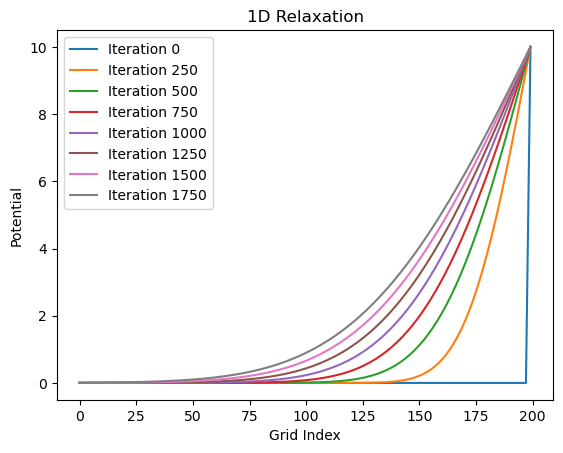
\includegraphics[keepaspectratio,alt={png}]{../images/activity-relaxation_2d_activity-relaxation_2d_tmp_9_0.png}}
\caption{png}
\end{figure}

It definitely looks like it gets close to the exact solution. But how
close? Let's plot the difference between the exact solution and the
solution from our relaxation algorithm. The code below computes the
exact solution and then plots the absolute value of the difference
between the two at each point on the grid.

\begin{Shaded}
\begin{Highlighting}[]
\KeywordTok{def}\NormalTok{ compute\_exact\_solution(grid, left\_bc, right\_bc):}
\NormalTok{    x }\OperatorTok{=}\NormalTok{ np.linspace(}\DecValTok{0}\NormalTok{, }\BuiltInTok{len}\NormalTok{(grid)}\OperatorTok{{-}}\DecValTok{1}\NormalTok{, }\BuiltInTok{len}\NormalTok{(grid))}
    \ControlFlowTok{return}\NormalTok{ left\_bc }\OperatorTok{+}\NormalTok{ x }\OperatorTok{*}\NormalTok{ (right\_bc }\OperatorTok{{-}}\NormalTok{ left\_bc) }\OperatorTok{/}\NormalTok{ (}\BuiltInTok{len}\NormalTok{(grid)}\OperatorTok{{-}}\DecValTok{1}\NormalTok{)}

\KeywordTok{def}\NormalTok{ plot\_error(stored\_iterations, exact\_solution):}
    
    \CommentTok{\# Plotting error}
\NormalTok{    final\_result }\OperatorTok{=}\NormalTok{ stored\_iterations[}\OperatorTok{{-}}\DecValTok{1}\NormalTok{]}
\NormalTok{    error }\OperatorTok{=}\NormalTok{ np.}\BuiltInTok{abs}\NormalTok{(final\_result }\OperatorTok{{-}}\NormalTok{ exact\_solution)}
\NormalTok{    plt.plot(error, label}\OperatorTok{=}\StringTok{"Error"}\NormalTok{, color}\OperatorTok{=}\StringTok{\textquotesingle{}red\textquotesingle{}}\NormalTok{)}
\NormalTok{    plt.legend()}
\NormalTok{    plt.xlabel(}\StringTok{\textquotesingle{}Grid Index\textquotesingle{}}\NormalTok{)}
\NormalTok{    plt.ylabel(}\StringTok{\textquotesingle{}Error\textquotesingle{}}\NormalTok{)}
\NormalTok{    plt.title(}\StringTok{\textquotesingle{}Error in 1D Relaxation\textquotesingle{}}\NormalTok{)}
\NormalTok{    plt.show()}
\end{Highlighting}
\end{Shaded}

\begin{Shaded}
\begin{Highlighting}[]
\NormalTok{exact\_solution }\OperatorTok{=}\NormalTok{ compute\_exact\_solution(grid, left\_bc, right\_bc)}
\NormalTok{plot\_error(stored\_iterations, exact\_solution)}
\end{Highlighting}
\end{Shaded}

\begin{figure}
\centering
\pandocbounded{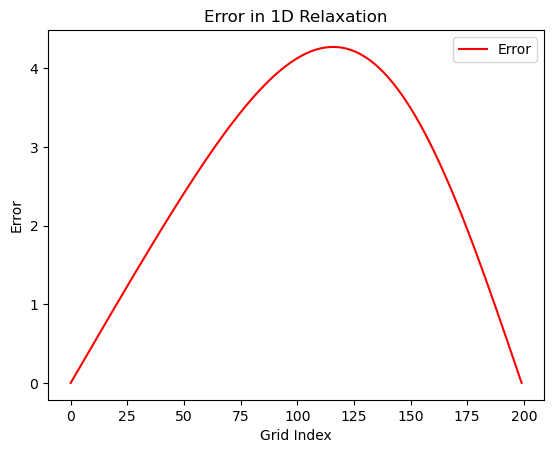
\includegraphics[keepaspectratio,alt={png}]{../images/activity-relaxation_2d_activity-relaxation_2d_tmp_12_0.png}}
\caption{png}
\end{figure}

\textbf{✅ Do this}

\begin{enumerate}
\def\labelenumi{\arabic{enumi}.}
\tightlist
\item
  Make sure you can run the code above and you have conceptual
  understanding of what it is doing. Test it and make sure it follows
  your intuition.
\item
  Modify the code to do a better job of predicting the exact solution.
  Get the maximum absolute error below 0.01, 0.001, 1e-4, 1e-5. How many
  iterations does it take to get to each of these values?
\item
  Modify the code to stop when the maximum absolute error is below a
  value of your choosing. Did you include a \texttt{max\_iterations}
  variable? If not, do so to avoid infinite loops.
\end{enumerate}

\subsection{2D Relaxation}\label{d-relaxation}

The 2D relaxation code is very similar to the 1D code. One difference is
that the grid has to be traversed in both directions. This means that
you will need to move systematically through the 2D grid. The second is
that you have to ensure the boundary conditions are set across the
entire edge of the grid.

We recommend breaking the approach into similar functions as above.

\begin{enumerate}
\def\labelenumi{\arabic{enumi}.}
\tightlist
\item
  Initialize the 2D grid of a chosen size (we've done that for you)
\item
  Set the boundary conditions (here you want a functions that can set
  each edge to a value or array of values) \emph{Hint: try using cases
  or if else to send edge information (`top', `left') and then use the
  \texttt{:} with the correct index to set the values for a full row or
  column (e.g., V{[}:,0{]})}
\item
  Relax the grid (here you will need to loop through the grid in both
  directions)
\end{enumerate}

We've started the code for you below. You will need to finish it.

\begin{Shaded}
\begin{Highlighting}[]
\KeywordTok{def}\NormalTok{ initialize\_grid\_2d(size):}
    \CommentTok{\textquotesingle{}\textquotesingle{}\textquotesingle{}Initialize the grid of potential values\textquotesingle{}\textquotesingle{}\textquotesingle{}}
    \ControlFlowTok{return}\NormalTok{ np.zeros((size, size))}

\KeywordTok{def}\NormalTok{ set\_boundary(phi, edge, value):}
    \CommentTok{\textquotesingle{}\textquotesingle{}\textquotesingle{}phi is the whole grid of potential values that you initialized}
\CommentTok{    edge is the edge of the grid that you want to set (top, bottom, left, right)}
\CommentTok{    value is the value you want to set the edge to (single number or array)\textquotesingle{}\textquotesingle{}\textquotesingle{}}

\KeywordTok{def}\NormalTok{ relax(phi, N, tolerance, max\_iterations}\OperatorTok{=}\DecValTok{10000}\NormalTok{, store\_frequency}\OperatorTok{=}\DecValTok{1000}\NormalTok{):}
    \CommentTok{\textquotesingle{}\textquotesingle{}\textquotesingle{}phi is the grid of potential values that you initialized}
\CommentTok{    after you set the boundary conditions. That is key!}
\CommentTok{    N is the size of the grid (assumed square}
\CommentTok{    tolerance is the stopping criterion {-} you control this; be careful}
\CommentTok{    max\_iterations is the maximum number of iterations to run (stops loop if not converged)}
\CommentTok{    store\_frequency is how often you want to store the phi values (for plotting)\textquotesingle{}\textquotesingle{}\textquotesingle{}}
    
\NormalTok{    iterations }\OperatorTok{=} \DecValTok{0} \CommentTok{\#\# Keep track of the number of iterations}
\NormalTok{    delta }\OperatorTok{=} \FloatTok{1.0} \CommentTok{\#\# Initialize delta (error) to be larger than tolerance}
    
\NormalTok{    stored\_phi }\OperatorTok{=}\NormalTok{ [] }\CommentTok{\#\# Keep track of phi values for plotting}
\NormalTok{    stored\_deltas }\OperatorTok{=}\NormalTok{ []  }\CommentTok{\#\# Keep track of delta values for plotting}
    
    \CommentTok{\#\# Loop condition to run until convergence or max\_iterations}
    \ControlFlowTok{while}\NormalTok{ delta }\OperatorTok{\textgreater{}}\NormalTok{ tolerance }\KeywordTok{and}\NormalTok{ iterations }\OperatorTok{\textless{}}\NormalTok{ max\_iterations:}
        \CommentTok{\# Store the old phi values to calculate delta later}
\NormalTok{        phi\_old }\OperatorTok{=}\NormalTok{ phi.copy()}
        
        \CommentTok{\#\#\#\#\#\#\#\#\#\#\#\#\#\#\#\#\#\#\#\#\#\#}
        \CommentTok{\#\#\# YOUR CODE HERE }\AlertTok{\#\#\#}
        \CommentTok{\#\#\#\#\#\#\#\#\#\#\#\#\#\#\#\#\#\#\#\#\#\#}
        
        \CommentTok{\# Calculate delta: max difference between new and old phi values}
\NormalTok{        delta }\OperatorTok{=}\NormalTok{ np.}\BuiltInTok{max}\NormalTok{(np.}\BuiltInTok{abs}\NormalTok{(phi }\OperatorTok{{-}}\NormalTok{ phi\_old))}
        
        \CommentTok{\#\# Increment the iteration counter}
\NormalTok{        iterations }\OperatorTok{+=} \DecValTok{1}
        
        \CommentTok{\#\# Store phi and delta values every store\_frequency iterations}
        \ControlFlowTok{if}\NormalTok{ iterations }\OperatorTok{\%}\NormalTok{ store\_frequency }\OperatorTok{==} \DecValTok{0}\NormalTok{:}
\NormalTok{            stored\_phi.append(phi.copy())}
\NormalTok{            stored\_deltas.append(delta)}
            \BuiltInTok{print}\NormalTok{(}\SpecialStringTok{f"Iteration: }\SpecialCharTok{\{}\NormalTok{iterations}\SpecialCharTok{\}}\SpecialStringTok{, Delta: }\SpecialCharTok{\{}\NormalTok{delta}\SpecialCharTok{\}}\SpecialStringTok{"}\NormalTok{)}
    
    \ControlFlowTok{return}\NormalTok{ stored\_phi, stored\_deltas, iterations}
\end{Highlighting}
\end{Shaded}

\textbf{✅ Do this}

Finish the 2D relaxation code (below we've written up an example use
case that it should work for) 1. You need to make sure the boundary
conditions are set correctly 2. You need to traverse the grid and
calculate the average of the neighboring points

It should be that once you have that working, the code below will run.
You will need to plot it to see if it is working correctly.

\begin{Shaded}
\begin{Highlighting}[]

\CommentTok{\# Example Usage}
\NormalTok{L }\OperatorTok{=} \FloatTok{1.0}
\NormalTok{h }\OperatorTok{=} \FloatTok{0.01}
\NormalTok{tolerance }\OperatorTok{=} \FloatTok{1e{-}5}
\NormalTok{N }\OperatorTok{=} \BuiltInTok{int}\NormalTok{(L}\OperatorTok{/}\NormalTok{h)}

\NormalTok{phi }\OperatorTok{=}\NormalTok{ initialize\_grid\_2d(N}\OperatorTok{+}\DecValTok{1}\NormalTok{)}

\CommentTok{\# Set varying potential on top boundary}
\NormalTok{x }\OperatorTok{=}\NormalTok{ np.linspace(}\DecValTok{0}\NormalTok{, L, N}\OperatorTok{+}\DecValTok{1}\NormalTok{)}
\NormalTok{V\_top }\OperatorTok{=} \DecValTok{10} \OperatorTok{*}\NormalTok{ np.sin(}\DecValTok{2} \OperatorTok{*}\NormalTok{ np.pi }\OperatorTok{*}\NormalTok{ x)}
\NormalTok{set\_boundary(phi, }\StringTok{\textquotesingle{}top\textquotesingle{}}\NormalTok{, V\_top)}

\CommentTok{\# Set constant potential on other boundaries}
\NormalTok{set\_boundary(phi, }\StringTok{\textquotesingle{}bottom\textquotesingle{}}\NormalTok{, }\DecValTok{0}\NormalTok{)}
\NormalTok{set\_boundary(phi, }\StringTok{\textquotesingle{}left\textquotesingle{}}\NormalTok{, }\DecValTok{5}\NormalTok{)}
\NormalTok{set\_boundary(phi, }\StringTok{\textquotesingle{}right\textquotesingle{}}\NormalTok{, }\DecValTok{5}\NormalTok{)}

\CommentTok{\# Relaxation}
\NormalTok{stored\_phi, stored\_deltas, iterations }\OperatorTok{=}\NormalTok{ relax(phi, N, tolerance)}
\BuiltInTok{print}\NormalTok{(}\SpecialStringTok{f"Converged in }\SpecialCharTok{\{}\NormalTok{iterations}\SpecialCharTok{\}}\SpecialStringTok{ iterations."}\NormalTok{)}
\end{Highlighting}
\end{Shaded}

\begin{verbatim}
Converged in 1 iterations.
\end{verbatim}

\subsection{What about Poisson's
equation?}\label{what-about-poissons-equation}

It turns out we can use a very similar approach when we have charges!
Alia has written up a script that implements the relaxation approach for
Poisson's equation. You can find it below along with the derivation.

\[\nabla^2 \phi = -\frac{\rho}{\epsilon_0}\]

Where \(\rho\) is a \textbf{charge density}.

Substituting our 2nd partial derivative equations gives us:

\[
\frac{\partial^2 \phi}{\partial x^2} + \frac{\partial^2 \phi}{\partial y^2}  = \frac{\phi(x+h,y) + \phi(x-h,y) - 2\phi(x,y) + \phi(x,y+h) + \phi(x,y-h) - 2\phi(x,y)}{h^2} = -\frac{\rho}{\epsilon_0}
\]

Which in turn gives us the update equation:

\[
\phi_{k+1}(x,y) = \frac{1}{4}\left[\phi_{k}(x+h,y) + \phi_{k}(x-h,y) + \phi_{k}(x,y+h) + \phi_{k}(x,y-h) \right] + \frac{h^2}{4\epsilon_0} \rho(x,y)
\]

We can implement this (warning: this takes a long time to converge).

\begin{Shaded}
\begin{Highlighting}[]
\CommentTok{\# constants and parameters}
\NormalTok{L }\OperatorTok{=} \DecValTok{1}
\NormalTok{h }\OperatorTok{=} \FloatTok{0.01}
\NormalTok{V }\OperatorTok{=} \DecValTok{1}
\NormalTok{N }\OperatorTok{=} \BuiltInTok{int}\NormalTok{(L}\OperatorTok{/}\FloatTok{0.01}\NormalTok{)}
\NormalTok{tol }\OperatorTok{=} \FloatTok{1e{-}2}
\NormalTok{epsilon0 }\OperatorTok{=} \FloatTok{8.854e{-}12}

\CommentTok{\# setup phi, phiprime arrays}
\NormalTok{phi }\OperatorTok{=}\NormalTok{ np.zeros((N}\OperatorTok{+}\DecValTok{1}\NormalTok{,N}\OperatorTok{+}\DecValTok{1}\NormalTok{))}
\NormalTok{phiprime }\OperatorTok{=}\NormalTok{ np.copy(phi) }\CommentTok{\# to play the part of phi (k+1)}

\KeywordTok{def}\NormalTok{ rho(i,j):}
\NormalTok{    x }\OperatorTok{=}\NormalTok{ i }\OperatorTok{*}\NormalTok{ h}
\NormalTok{    y }\OperatorTok{=}\NormalTok{ j }\OperatorTok{*}\NormalTok{ h}
    \ControlFlowTok{if}\NormalTok{ x }\OperatorTok{\textgreater{}=} \FloatTok{0.6} \KeywordTok{and}\NormalTok{ x }\OperatorTok{\textless{}=} \FloatTok{0.8} \KeywordTok{and}\NormalTok{ y }\OperatorTok{\textgreater{}=} \FloatTok{0.2} \KeywordTok{and}\NormalTok{ y }\OperatorTok{\textless{}=} \FloatTok{0.4}\NormalTok{:}
        \ControlFlowTok{return} \FloatTok{1e{-}7}
    \ControlFlowTok{elif}\NormalTok{ x }\OperatorTok{\textgreater{}=} \FloatTok{0.2} \KeywordTok{and}\NormalTok{ x }\OperatorTok{\textless{}=} \FloatTok{0.4} \KeywordTok{and}\NormalTok{ y }\OperatorTok{\textgreater{}=} \FloatTok{0.6} \KeywordTok{and}\NormalTok{ y }\OperatorTok{\textless{}=} \FloatTok{0.8}\NormalTok{:}
        \ControlFlowTok{return} \OperatorTok{{-}}\FloatTok{1e{-}7}
    \ControlFlowTok{else}\NormalTok{:}
        \ControlFlowTok{return} \FloatTok{0.}

\NormalTok{k }\OperatorTok{=} \DecValTok{0} \CommentTok{\# track number of iterations}
\NormalTok{delta }\OperatorTok{=} \FloatTok{1.0} \CommentTok{\# initial delta}

\ControlFlowTok{while}\NormalTok{ delta }\OperatorTok{\textgreater{}}\NormalTok{ tol: }\CommentTok{\# run until converged}

    \ControlFlowTok{for}\NormalTok{ i }\KeywordTok{in} \BuiltInTok{range}\NormalTok{(N}\OperatorTok{+}\DecValTok{1}\NormalTok{):}
        \ControlFlowTok{for}\NormalTok{ j }\KeywordTok{in} \BuiltInTok{range}\NormalTok{(N}\OperatorTok{+}\DecValTok{1}\NormalTok{):}
            \ControlFlowTok{if}\NormalTok{ i }\OperatorTok{==} \DecValTok{0} \KeywordTok{or}\NormalTok{ i }\OperatorTok{==}\NormalTok{ N }\KeywordTok{or}\NormalTok{ j }\OperatorTok{==} \DecValTok{0} \KeywordTok{or}\NormalTok{  j }\OperatorTok{==}\NormalTok{ N: }\CommentTok{\# don\textquotesingle{}t update boundary}
\NormalTok{                phiprime[i,j] }\OperatorTok{=}\NormalTok{ phi[i,j]}
            \ControlFlowTok{else}\NormalTok{:}
                \CommentTok{\# relaxation update equation}
\NormalTok{                phiprime[i,j] }\OperatorTok{=} \FloatTok{0.25} \OperatorTok{*}\NormalTok{ (phi[i}\OperatorTok{+}\DecValTok{1}\NormalTok{,j] }\OperatorTok{+}\NormalTok{ phi[i}\OperatorTok{{-}}\DecValTok{1}\NormalTok{,j] }\OperatorTok{+}\NormalTok{ phi[i,j}\OperatorTok{+}\DecValTok{1}\NormalTok{] }\OperatorTok{+}\NormalTok{ phi[i,j}\OperatorTok{{-}}\DecValTok{1}\NormalTok{]) }\OperatorTok{+}\NormalTok{ h}\OperatorTok{**}\DecValTok{2} \OperatorTok{/}\NormalTok{ (}\DecValTok{4} \OperatorTok{*}\NormalTok{ epsilon0) }\OperatorTok{*}\NormalTok{ rho(i,j)}

    \CommentTok{\# find max difference for delta}
\NormalTok{    delta }\OperatorTok{=}\NormalTok{ np.}\BuiltInTok{abs}\NormalTok{(phi}\OperatorTok{{-}}\NormalTok{phiprime).}\BuiltInTok{max}\NormalTok{()}

    \CommentTok{\# swap arrays to keep iterating}
\NormalTok{    phi,phiprime }\OperatorTok{=}\NormalTok{ phiprime,phi }
    
    \CommentTok{\# track iterations}
\NormalTok{    k }\OperatorTok{+=} \DecValTok{1}
    \ControlFlowTok{if}\NormalTok{ k}\OperatorTok{\%}\DecValTok{500} \OperatorTok{==} \DecValTok{0} \KeywordTok{or}\NormalTok{ k }\OperatorTok{==}\DecValTok{1}\NormalTok{:}
        \BuiltInTok{print}\NormalTok{(}\StringTok{"iter:"}\NormalTok{,k,}\StringTok{"delta:"}\NormalTok{,delta)         }
\NormalTok{    delta }\OperatorTok{=}\NormalTok{ np.}\BuiltInTok{abs}\NormalTok{(phi}\OperatorTok{{-}}\NormalTok{phiprime).}\BuiltInTok{max}\NormalTok{()}

\BuiltInTok{print}\NormalTok{(k)}
\NormalTok{plt.imshow(phi)}
\NormalTok{plt.show()}
\end{Highlighting}
\end{Shaded}

\begin{verbatim}
iter: 1 delta: 0.28235825615541005
iter: 500 delta: 0.06832141135411973
iter: 1000 delta: 0.03251014051510026
iter: 1500 delta: 0.017114857647044346
1931
\end{verbatim}

\begin{figure}
\centering
\pandocbounded{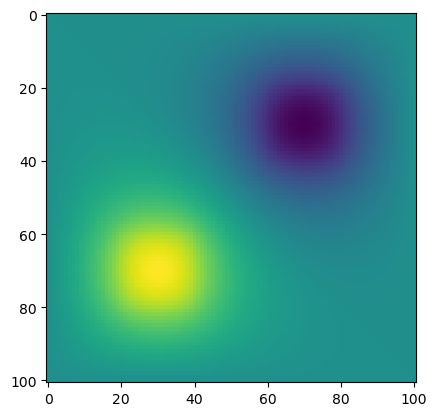
\includegraphics[keepaspectratio,alt={png}]{../images/activity-relaxation_2d_activity-relaxation_2d_tmp_19_1.png}}
\caption{png}
\end{figure}
